\section{Run time and memory before and after}
\label{sec:sequential}

\subsection{Method}

Table~\ref{tab:environments} lists the machines the measurements in this report come from.
The sequential measurements were taken on \SequentialMachine. For each matrix size the
assignment program was built twice from the same source, once against the original library
and once against the cached one, and run on one core. A small launcher starts the program
and reads its wall-clock time and its peak resident memory from the operating system when
it exits. The identity $\det(C) = \det(A)\det(B)$ was verified by the program in every run.
Every table and figure in this report is generated from the recorded result files by a
script in the repository.

\begin{table}[t]
  \caption{Machines used for the measurements.}
  \label{tab:environments}
  \centering
  \footnotesize
  \begin{tabular}{@{}l p{3.0cm} p{3.6cm}@{}}
\toprule
Label & Processor and memory & Software \\
\midrule
cloud-vm & Intel Xeon Processor @ 2.10GHz, 2 CPUs, 7.8 GiB & Ubuntu 24.04.5 LTS (virtual machine); GCC 13.3.0; Open MPI 4.1.6 \\
\bottomrule
\end{tabular}

\end{table}

\subsection{Results}

Table~\ref{tab:sequential} and Fig.~\ref{fig:runtime} give the run times. At
$N = \SeqLargestBoth$, the largest size we ran with both libraries, the original takes
\SeqOriginalAtLargest{} and the cached version \SeqCachedAtLargest, a factor of
\SeqSpeedupAtLargest. The largest cached run, $N = \SeqLargestCached$, takes
\SeqCachedAtLargestCached.

Table~\ref{tab:machines} gives the same comparison for every machine the program was run on, at the largest size each of them ran with both libraries.

\begin{table}[t]
  \caption{Original and cached finite field on each machine.}
  \label{tab:machines}
  \centering
  \footnotesize
  \setlength{\tabcolsep}{4pt}
\begin{tabular}{@{}l r r r r r r@{}}
\toprule
& & \multicolumn{3}{c}{Run time (s)} & \multicolumn{2}{c}{Memory (MiB)} \\
\cmidrule(lr){3-5}\cmidrule(l){6-7}
Machine & $N$ & Original & Cached & Speedup & Original & Cached \\
\midrule
cloud-vm & 1000 & 819 & 37.6 & 21.8$\times$ & 217 & 18.4 \\
lemmen & 1000 & 378 & 15.3 & 24.7$\times$ & 218 & 18.6 \\
\bottomrule
\end{tabular}
\end{table}


\begin{table}[t]
  \caption{The assignment program with the original and the cached finite field on
  \SequentialMachine. A dash marks a size that was not run. Where a size was run more than
  once, the median is given.}
  \label{tab:sequential}
  \centering
  \footnotesize
  \begin{tabular}{@{}r r r r r r@{}}
\toprule
& \multicolumn{3}{c}{Run time (s)} & \multicolumn{2}{c}{Peak memory (MiB)} \\
\cmidrule(lr){2-4}\cmidrule(l){5-6}
$N$ & Original & Cached & Speedup & Original & Cached \\
\midrule
100 & 0.374 & 0.295 & 1.3$\times$ & 6.2 & 11.4 \\
200 & 2.91 & 0.514 & 5.7$\times$ & 12.7 & 11.5 \\
400 & 23.5 & 1.25 & 18.8$\times$ & 38.3 & 12.2 \\
800 & 190 & 7.60 & 25.0$\times$ & 141 & 15.8 \\
1000 & 378 & 15.3 & 24.7$\times$ & 218 & 18.6 \\
2000 & -- & 147 & -- & -- & 41.2 \\
4000 & -- & 1\,182 & -- & -- & 133 \\
\bottomrule
\end{tabular}

\end{table}

\begin{figure}[t]
  \centering
  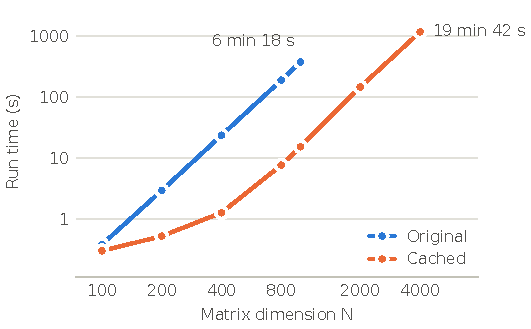
\includegraphics[width=\columnwidth]{figures/runtime.pdf}
  \caption{Run time of the whole program against matrix dimension, on logarithmic axes.}
  \label{fig:runtime}
\end{figure}

The gain grows with the matrix (Fig.~\ref{fig:speedup}), and
\SeqSmallestSentence. The reason is the first use of each operand pair.
Fig.~\ref{fig:cache} shows how the tables fill. At $N = 100$ only
\CacheHitAtHundred\% of the additions and multiplications are answered from a table, and the
rest still run the original arithmetic once. The share passes 99\% at
$N = \CacheHitNinetyNineSize$.

\begin{figure}[t]
  \centering
  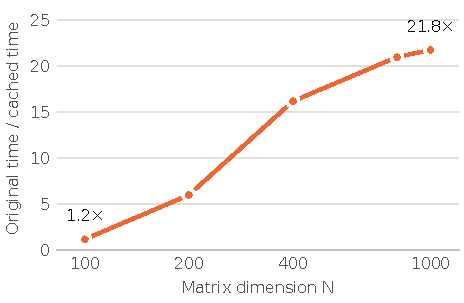
\includegraphics[width=\columnwidth]{figures/speedup.pdf}
  \caption{Speedup of the cached program over the original.}
  \label{fig:speedup}
\end{figure}

\begin{figure}[t]
  \centering
  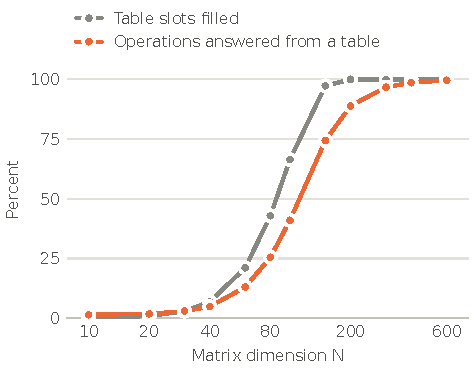
\includegraphics[width=\columnwidth]{figures/cache_fill.pdf}
  \caption{Cache behaviour over one run of the program: the share of the addition and
  multiplication table slots that end up filled, and the share of additions and
  multiplications answered from a table.}
  \label{fig:cache}
\end{figure}

\subsection{Memory}

The original library stores every matrix entry as a vector object that points to a
separate heap block. Measured from the growth of peak memory with $N$, that costs about
\SeqOriginalBytesPerEntry~bytes per entry on this system. The cached entry is two bytes.
Fig.~\ref{fig:memory} shows the effect. At $N = \SeqLargestBoth$ peak memory falls from
\SeqOriginalMemoryAtLargest{} to \SeqCachedMemoryAtLargest. The tables are a fixed cost of
about 7~MB. \SeqMemoryCrossoverSentence. At $N = \SeqLargestCached$ the cached program peaks
at \SeqCachedMemoryAtLargestCached.

\begin{figure}[t]
  \centering
  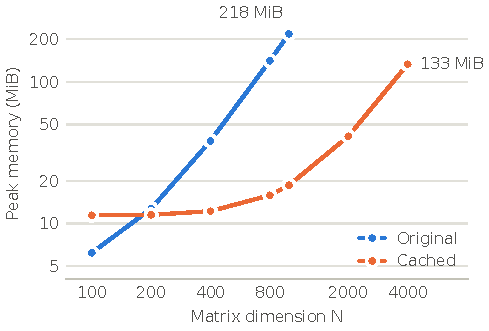
\includegraphics[width=\columnwidth]{figures/memory.pdf}
  \caption{Peak resident memory against matrix dimension, on logarithmic axes.}
  \label{fig:memory}
\end{figure}

\subsection{Where the remaining time goes}

Table~\ref{tab:phases} splits the largest run of each library into the matrix product and
the three determinants. With the cached library the product takes \SeqCachedProductShare\%
of the run, against \SeqOriginalProductShare\% with the original. The product accumulates each entry as a running
sum, so every table lookup for an addition has to wait for the previous one, which is the
chained pattern of Fig.~\ref{fig:lookup}. In the elimination the additions do not depend on
each other and the processor overlaps them.

\begin{table}[t]
  \caption{Time in the matrix product and in the three determinants, for the largest run
  of each library.}
  \label{tab:phases}
  \centering
  \footnotesize
  \begin{tabular}{@{}l r r r r@{}}
\toprule
Library & $N$ & Product (s) & Three det. (s) & Product share \\
\midrule
Original & 1000 & 425 & 393 & 52\% \\
Cached & 4000 & 2\,280 & 345 & 87\% \\
\bottomrule
\end{tabular}

\end{table}

\subsection{Comparison with the assignment's figures}

Table~\ref{tab:reference} sets our measurements beside the figures in the assignment text,
which come from a different machine. \SeqReferenceNote

\begin{table}[t]
  \caption{The assignment's reference figures (Apple M3 Max) and our measurements on
  \SequentialMachine.}
  \label{tab:reference}
  \centering
  \footnotesize
  \begin{tabular}{@{}r l r r r r@{}}
\toprule
& & \multicolumn{2}{c}{Assignment text} & \multicolumn{2}{c}{Measured here} \\
\cmidrule(lr){3-4}\cmidrule(l){5-6}
$N$ & Library & Time & Memory & Time & Memory \\
\midrule
4000 & Original & 6 h 40 min & 2.6 GB & -- & -- \\
4000 & Cached & 20 min 16 s & 0.53 GB & 43 min 48 s & 0.13 GiB \\
6000 & Original & 22 h 30 min & 5.8 GB & -- & -- \\
6000 & Cached & 1 h 08 min & 1.2 GB & -- & -- \\
\bottomrule
\end{tabular}

\end{table}
